\documentclass[a4paper,11pt]{article}
\usepackage{amsmath}
\usepackage{amssymb}
\usepackage{placeins}
\usepackage{array}
\usepackage{hyperref}
\usepackage{graphicx}
\usepackage{units}
\usepackage{xfrac}
\usepackage[version=4]{mhchem}
\usepackage[margin=0.9in]{geometry,caption}
\usepackage{braket}
\usepackage{gensymb}
\usepackage{wasysym}
\usepackage{tikz}
\usepackage{physics}
\usepackage{booktabs}
\usepackage{multirow}
\usepackage{subcaption}
\usepackage[capitalise,
					 noabbrev]{cleveref}
\usepackage[mathlines]{lineno}
\usepackage{cleveref}
 \usepackage{setspace}
 \usepackage{bm}
\usepackage{fancyhdr}
\usepackage{makecell}
\usepackage{setspace}
\usepackage{chngcntr}
\usepackage{afterpage}
\usepackage{bm}
\usepackage{tocloft}
\setlength{\cfttabnumwidth}{1.5cm}
\setlength{\cftfignumwidth}{1.5cm}

\renewcommand*\thetable{\Roman{table}}


%%%Add this for version history
%\setcounter{section}{-1}

%%spacing on tilde for approximate values
\let\oldsim\sim 
\renewcommand{\sim}{{\oldsim}}

%%1.5 spacing
\onehalfspacing

\pagestyle{fancy}
\fancyhf{}
\setlength{\headheight}{14pt}
\fancyhead[L]{\nouppercase\leftmark}
\fancyhead[L]{\nouppercase\rightmark}
%\fancyhead[ER,OL]{\nouppercase\rightmark}
\rhead{\thepage}


%%%Patch AMSmath environments to work correctly with lineno
\usepackage{etoolbox}
\newcommand*\linenomathpatchAMS[1]{%
  \expandafter\pretocmd\csname #1\endcsname {\linenomathAMS}{}{}%
  \expandafter\pretocmd\csname #1*\endcsname{\linenomathAMS}{}{}%
  \expandafter\apptocmd\csname end#1\endcsname {\endlinenomath}{}{}%
  \expandafter\apptocmd\csname end#1*\endcsname{\endlinenomath}{}{}%
}

\expandafter\ifx\linenomath\linenomathWithnumbers
  \let\linenomathAMS\linenomathWithnumbers
  %% The following line gets rid of an extra line numbers at the bottom:
  \patchcmd\linenomathAMS{\advance\postdisplaypenalty\linenopenalty}{}{}{}
\else
  \let\linenomathAMS\linenomathNonumbers
\fi
\linenomathpatchAMS{align}

\graphicspath{{images/}}

\begin{document}

\title{\huge{HK-TN-???: HK LI Fibre Specifications}}
\author{S. J. Jenkins, B. Bogdan, N. Foster, N. K. McCauley}

\maketitle

\tableofcontents

\newpage

\section{Introduction}
The Hyper-Kamiokande experiment has a broad physics program, including the aim of making precision measurements of neutrino oscillation parameters. In order to make such precision measurements, a precise understanding of the detector itself is required. To this end an array of different calibration systems are planned, with each playing a crucial role in driving systematic uncertainties down to the percent-level required.

A key component of the calibration program is the light injection (LI) system, which has two primary aims. The first is to measure the optical properties of the water in the tank, and monitor how the measured absorption and scattering parameters evolve with time. The second is to provide light sources with which to calibrate PMT response. In order to illuminate the injectors, lengths of fibre optic cable will be used to carry light from the sources on the top of the tank, all the way to the injectors installed on the PMT support structure.

This technical note focuses on the fibre optic requirements for the LI system, describing the quantities and lengths of cables needed, along with the lab measurements performed to decide on which types of fibre optic cables to use.

\section{HK LI System Overview}

The HK LI system will be split into two parts, one for the inner detector (ID) and one for the outer detector (OD). The ID system will consist of 33 injector positions, each housing a diffuser and collimator. Full details of the diffuser and collimator designs and requirements can be found in HK-TN-0042 \cite{bib:tn0042} and HK-TN-0065 \cite{bib:tn0065}, respectively. 28 injector positions will be located in the barrel region, with 7 locations equally spaced in $z$, each having four positions equally spaced in $\theta$. The bottom end-cap will feature four more injector locations, with the injectors all facing upwards in the $+z$ direction. The top end-cap will feature a single location, where a calibration port will be used, rather than fixing to the PMT support structure.{\color{red} confirm if we'll have a top collimator} \cref{fig:IDmap} shows the injector locations described.
\begin{figure}[h]
\centering
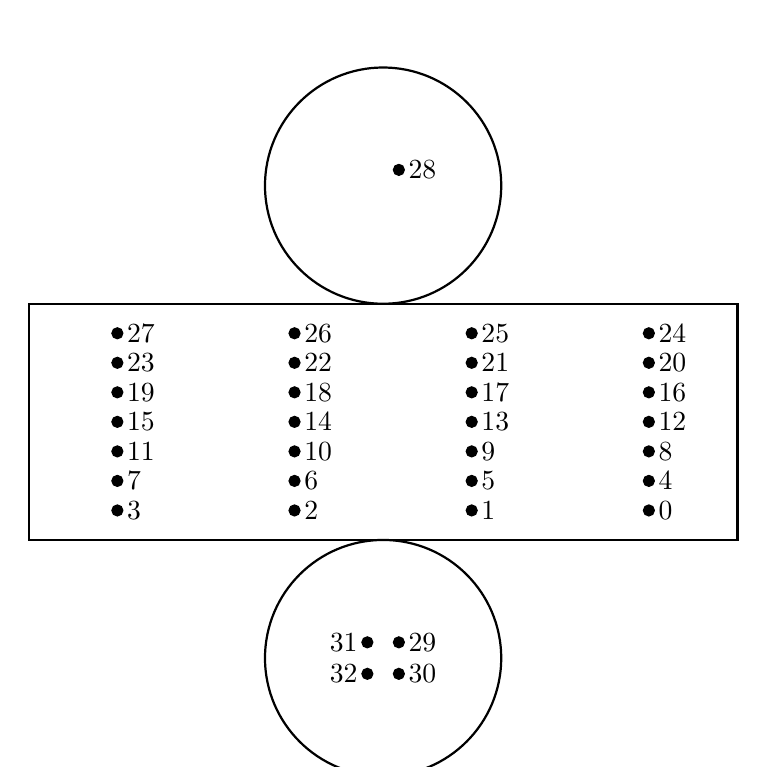
\begin{tikzpicture}
\draw[thick] (-4.5, -1.5) rectangle (4.5, 1.5);
\draw[thick] (0, 3) circle (1.5cm);
\draw[thick] (0, -3) circle (1.5cm);
\filldraw[black] (3.375, -1.125) circle (2pt) node[anchor=west]{0};
\filldraw[black] (3.375, -0.75) circle (2pt) node[anchor=west]{4};
\filldraw[black] (3.375, -0.375) circle (2pt) node[anchor=west]{8};
\filldraw[black] (3.375, 0) circle (2pt) node[anchor=west]{12};
\filldraw[black] (3.375, 0.375) circle (2pt) node[anchor=west]{16};
\filldraw[black] (3.375, 0.75) circle (2pt) node[anchor=west]{20};
\filldraw[black] (3.375, 1.125) circle (2pt) node[anchor=west]{24};
\filldraw[black] (1.125, -1.125) circle (2pt) node[anchor=west]{1};
\filldraw[black] (1.125, -0.75) circle (2pt) node[anchor=west]{5};
\filldraw[black] (1.125, -0.375) circle (2pt) node[anchor=west]{9};
\filldraw[black] (1.125, 0) circle (2pt) node[anchor=west]{13};
\filldraw[black] (1.125, 0.375) circle (2pt) node[anchor=west]{17};
\filldraw[black] (1.125, 0.75) circle (2pt) node[anchor=west]{21};
\filldraw[black] (1.125, 1.125) circle (2pt) node[anchor=west]{25};
\filldraw[black] (-3.375, -1.125) circle (2pt) node[anchor=west]{3};
\filldraw[black] (-3.375, -0.75) circle (2pt) node[anchor=west]{7};
\filldraw[black] (-3.375, -0.375) circle (2pt) node[anchor=west]{11};
\filldraw[black] (-3.375, 0) circle (2pt) node[anchor=west]{15};
\filldraw[black] (-3.375, 0.375) circle (2pt) node[anchor=west]{19};
\filldraw[black] (-3.375, 0.75) circle (2pt) node[anchor=west]{23};
\filldraw[black] (-3.375, 1.125) circle (2pt) node[anchor=west]{27};
\filldraw[black] (-1.125, -1.125) circle (2pt) node[anchor=west]{2};
\filldraw[black] (-1.125, -0.75) circle (2pt) node[anchor=west]{6};
\filldraw[black] (-1.125, -0.375) circle (2pt) node[anchor=west]{10};
\filldraw[black] (-1.125, 0) circle (2pt) node[anchor=west]{14};
\filldraw[black] (-1.125, 0.375) circle (2pt) node[anchor=west]{18};
\filldraw[black] (-1.125, 0.75) circle (2pt) node[anchor=west]{22};
\filldraw[black] (-1.125, 1.125) circle (2pt) node[anchor=west]{26};
\filldraw[black] (0.2, 3.2) circle (2pt) node[anchor=west]{28};
\filldraw[black] (0.2, -2.8) circle (2pt) node[anchor=west]{29};
\filldraw[black] (0.2, -3.2) circle (2pt) node[anchor=west]{30};
\filldraw[black] (-0.2, -2.8) circle (2pt) node[anchor=east]{31};
\filldraw[black] (-0.2, -3.2) circle (2pt) node[anchor=east]{32};
\end{tikzpicture}
\caption{Injector location map for ID positions. Each location will feature a diffuser and collimator.}\label{fig:IDmap}
\end{figure}
Installing injectors at different heights throughout the detector will allow water parameters to be measured as a function of depth.

The OD system will consist primarily of diffusers, using bare hemispheres coupled to fibres, rather than the housed versions used for the ID system. 122 of these OD diffusers will be installed, with the current design featuring 84 equally spaced around the barrel region. This results in 7 rows of 12 diffusers, with rows alternately offset from one another. This configuration is particularly advantageous as it matches the number of rows in the ID system, simplifying the installation of the fibre optic cables. Each end-cap would then feature 19 diffusers, again equally spaced across the surface. A diagram showing this layout is presented in \cref{fig:ODdiffmap}. Finally, 12 collimators will be installed in the OD, in suitable locations to achieve long path lengths such as across the end caps and up the side of the barrel. These collimators will be exactly the same as those installed in the ID.

\begin{figure}[h]
\centering
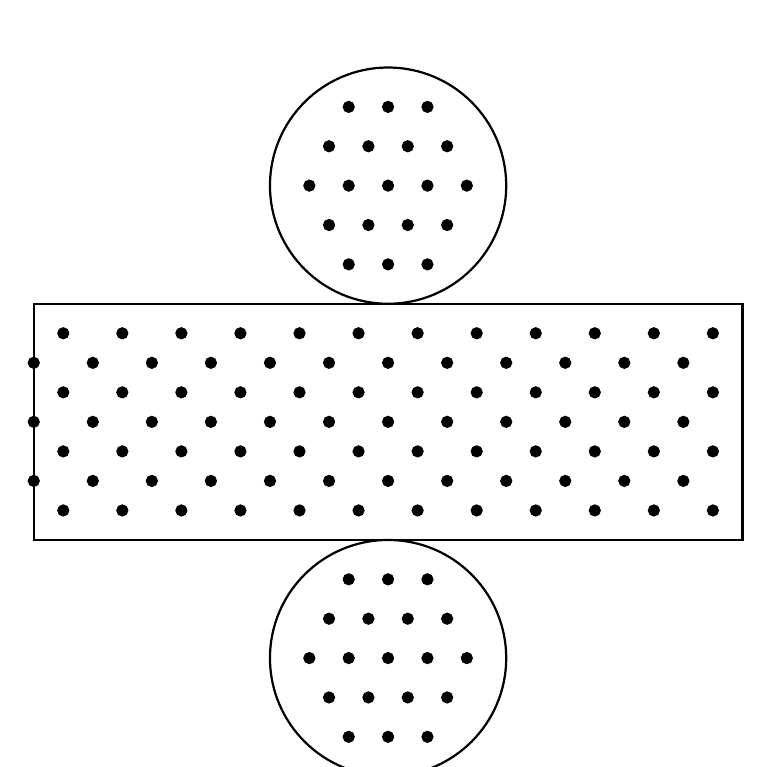
\begin{tikzpicture}
\draw[thick] (-4.5, -1.5) rectangle (4.5, 1.5);
\draw[thick] (0, 3) circle (1.5cm);
\draw[thick] (0, -3) circle (1.5cm);
%barrel locations
\foreach \x in {0,...,11}{
	\foreach \y in {0,...,6}{
		\ifodd \y \filldraw[black] (-4.5+\x*2*0.375, -1.125+\y*0.375) circle (2pt);
		\else \filldraw[black] (-4.5+0.375+\x*2*0.375, -1.125+\y*0.375) circle (2pt);
		\fi
		}
	}
%topcap
\foreach \y in {0,...,2}{
	\foreach \x in {0,...,2}{
		\filldraw[black] (-0.5+\x*0.5, 1.5+0.5+2*\y*0.5) circle (2pt);
		}
	}
\foreach \y in {0,...,1}{
	\foreach \x in {0,...,3}{
		\filldraw[black] (-0.75+\x*0.5, 1.5+2*0.5+2*\y*0.5) circle (2pt);
		}
	}
\foreach \x in {0,...,1}{
	\filldraw[black] (-1+\x*2, 3) circle (2pt);
	}
%bottom cap
\foreach \y in {0,...,2}{
	\foreach \x in {0,...,2}{
		\filldraw[black] (-0.5+\x*0.5, -1.5-0.5-2*\y*0.5) circle (2pt);
		}
	}
\foreach \y in {0,...,1}{
	\foreach \x in {0,...,3}{
		\filldraw[black] (-0.75+\x*0.5, -1.5-2*0.5-2*\y*0.5) circle (2pt);
		}
	}
\foreach \x in {0,...,1}{
	\filldraw[black] (-1+\x*2, -3) circle (2pt);
	}
\end{tikzpicture}
\caption{Injector location map for OD diffuser positions. Locations are approximate and dependent on PMT/WLS plate locations.}\label{fig:ODdiffmap}
\end{figure}


\section{Fibre Length Requirements}

\section{Fibre Lab Measurements}

\subsection{Fibre Test Stand}

\subsection{Attenuation Measurements}

\subsection{Dispersion Measurements}

\section{Summary}

\newpage
\begin{thebibliography}{99}

%%diffuser TN
\bibitem{bib:tn0042}
S. Boyd {\it et al.}, Hyper-Kamiokande Light Injector Diffuser Technical Note (HK-TN-0042)

%%collimator TN
\bibitem{bib:tn0065}
S. Boyd {\it et al.}, Hyper-Kamiokande Light Injector Collimator Technical Note (HK-TN-0065)

\end{thebibliography}

\end{document}